\subsection{Méthode de modélisation}
      \paragraph{}
      Afin de modéliser les fonctionnalités de notre solution, nous avons choisi le langage UML \textit{Unified Modeling Language} \cite{I}. Issu d’un large consensus, le langage UML garantit la stabilité et la performance d’un projet grâce à son caractère formel et industrialisé. Aussi facilite-t-il la compréhension du système par l’usage de représentations graphiques appelées diagrammes. Ces diagrammes nous ont permis de modéliser notre solution en utilisant les diagrammes de cas d’utilisation et de séquence.\\ \\
\subsection{Diagramme de cas d'utilisation}
    \paragraph{}
	  Le diagramme de cas d'utilisation représente la structure des grandes fonctionnalités nécessaires aux
    utilisateurs du système. C'est le premier diagramme du modèle UML, celui où s'assure la relation entre l'utilisateur et les objets que le système met en œuvre. 

	  \begin{figure}[H]
		     \begin{center}
			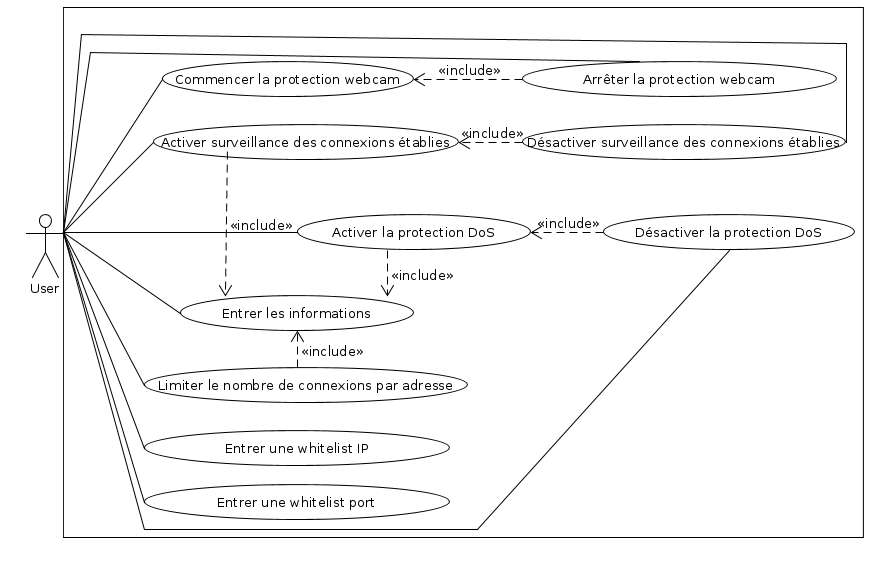
\includegraphics[scale=0.5]{images/use_case.png}
		     \end{center}
		     \caption{Diagramme de cas d'utilisation}
		     \label{Diagramme de cas d'utilisation}
	  \end{figure}
	  
	  Les informations à entrer désignent les identifiants que l'utilisateur doit entrer au début du programme. Ces derniers sont, en particulier, son nom, son email, son numéro de téléphone, son nom d'utilisateur \textbf{root} et le mot de passe associé. Le système se servira de cela pour lui envoyer des alertes et effectuer des tâches réservées à un utilisateur root.
\subsection{Diagramme de séquence}
 \paragraph{}
	  Le diagramme de séquence représente la succession chronologique des opérations réalisées par un acteur. Ce mode de représentation effectue la description du fonctionnement dynamique du système. En d'autres termes, il indique les objets que l'acteur va manipuler et les opérations qui font passer d'un objet à l'autre.
	  \begin{figure}[H]
		     \begin{center}
			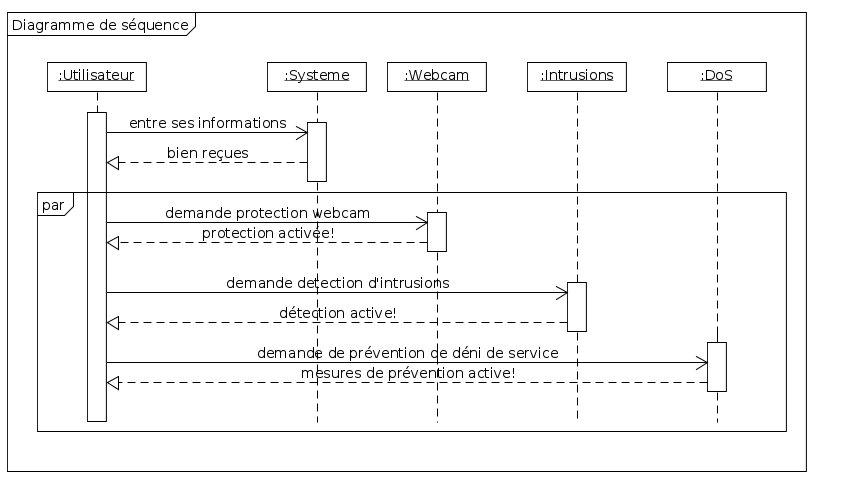
\includegraphics[scale=0.5]{images/sequence.png}
		     \end{center}
		     \caption{Diagramme de séquence}
		     \label{Diagramme de cas d'utilisation}
	  \end{figure}
	  Après que l'utilisateur ait entré ses informations, identifiants pour être administrateur de son système, il peut parallèlement activer la protection webcam, lancer la detection d'intrusion ou prévenir les dénis de service.